\documentclass[tikz, border=0pt]{standalone}
\usepackage{tikz}
\usetikzlibrary{arrows,automata,positioning}

\begin{document}
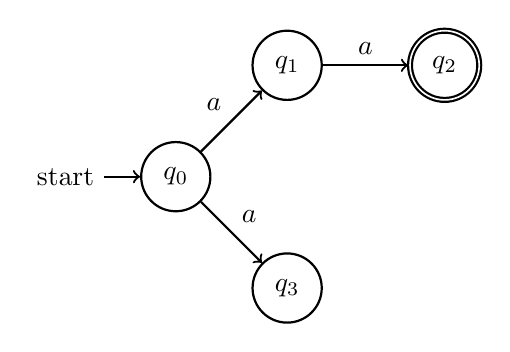
\begin{tikzpicture}[node distance=2cm, thick, auto]
% draw the states
\node[state, initial] (q_0) {\(q_0\)};
\node[state] (q_1) [above right of=q_0] {\(q_1\)};
\node[state, accepting] (q_2) [right of=q_1] {\(q_2\)};
\node[state] (q_3) [below right of=q_0] {\(q_3\)};
% draw the edges
\path[->] 
(q_0) edge node {\(a\)} (q_1)
(q_0) edge node {\(a\)} (q_3)
(q_1) edge node {\(a\)} (q_2)
;
\end{tikzpicture}
\end{document}